\section{A Constructed Formula for the Snipped N-Units Away Curve}

When we first defined the Snipped $N$-Units Away Curve in section 5, we took it as an assumption that it was a function $``f_N''(x)$ on $x$ from $\mathbb{R} \xrightarrow{} \mathbb{R}$. How do we know it is necessarily defined on all of $\mathbb{R}$? $\forall$ values of $x$m there is an associated point on the regular $N$-Unis Away Curve which we know never has an $x$-value location outside of $(x-N, x+N)$. Take some arbitrary extremely negative $x$-value $x_L$ and an arbitrary extremely positive $x$-value $x_R$. We know $\exists$ two points on the $N$-Units Away Curve that are on $(x_L - N, x_L + N)$ and $(x_R - N, x_R + N)$ respectively. As the $N$-Units Away Curve has parametric continuity, we know it has no gaps. It necessarily crosses all $x$ values between $x_L + N$ and $x_R - N$, and we  may place those as far off towards the two infinities as we would like. The Snipped $N$-Units Away Curve is necessarily defined on all of $\mathbb{R}$.

How can we possibly learn more about this function $``f_N''(x)$? Well, we know from the previous section that the Snipped $N$-Units Away Curve is precisely the point that a marble of radius $N$'s centerpoint would follow were it to roll along the function (assume for a positive $N$).

\begin{wrapfigure}{l}{0.25\textwidth}
  \includegraphics[width=.9\linewidth]{constructed-formula-img/Fig 10-33.png}
  \caption{Caption}
  \label{fig:fig10-33}
\end{wrapfigure}

Consider the following... Choose your favorite value $x = x_o$. Take a marble of radius $N$ and gradually lower it down towards the function. The moment it first contacts the function $y = f(x)$, stop right there. This is exactly the location that the marble would assume were it rolling along the function at $x = x_o$. The $y$-value of the centerpoint right there is thus equal to $``f_N'(x_o)$.

Let's rewind a bit and think through this more mathematically. Take your function $y = f(x)$ and suspend a marble of radius $N$ way up above the curve directly above $\exists x = x_o$. This circle has equation $(y - y_c)^2 + (x - x_o)^2 = N^2$, where $y_c$ us the moveable height of the centerpoint of the marble. Solving for $y$, we get that the bottom half of the semi-circle of the marble can be described by $y = - \sqrt{N^2 -(x - x_o)^2} + y_c$. What we seek is the very highest $y_c$ value $\ni$ the function and this bottom half of the marble touch, aka what is the highest possible $y_c \ni (- \sqrt{N^2 - (x - x_o)^2} + y_c) - f(x)$ has a zero on interval $x \in (x_o - N, x_o + N)$?

\begin{wrapfigure}{l}{0.25\textwidth}
  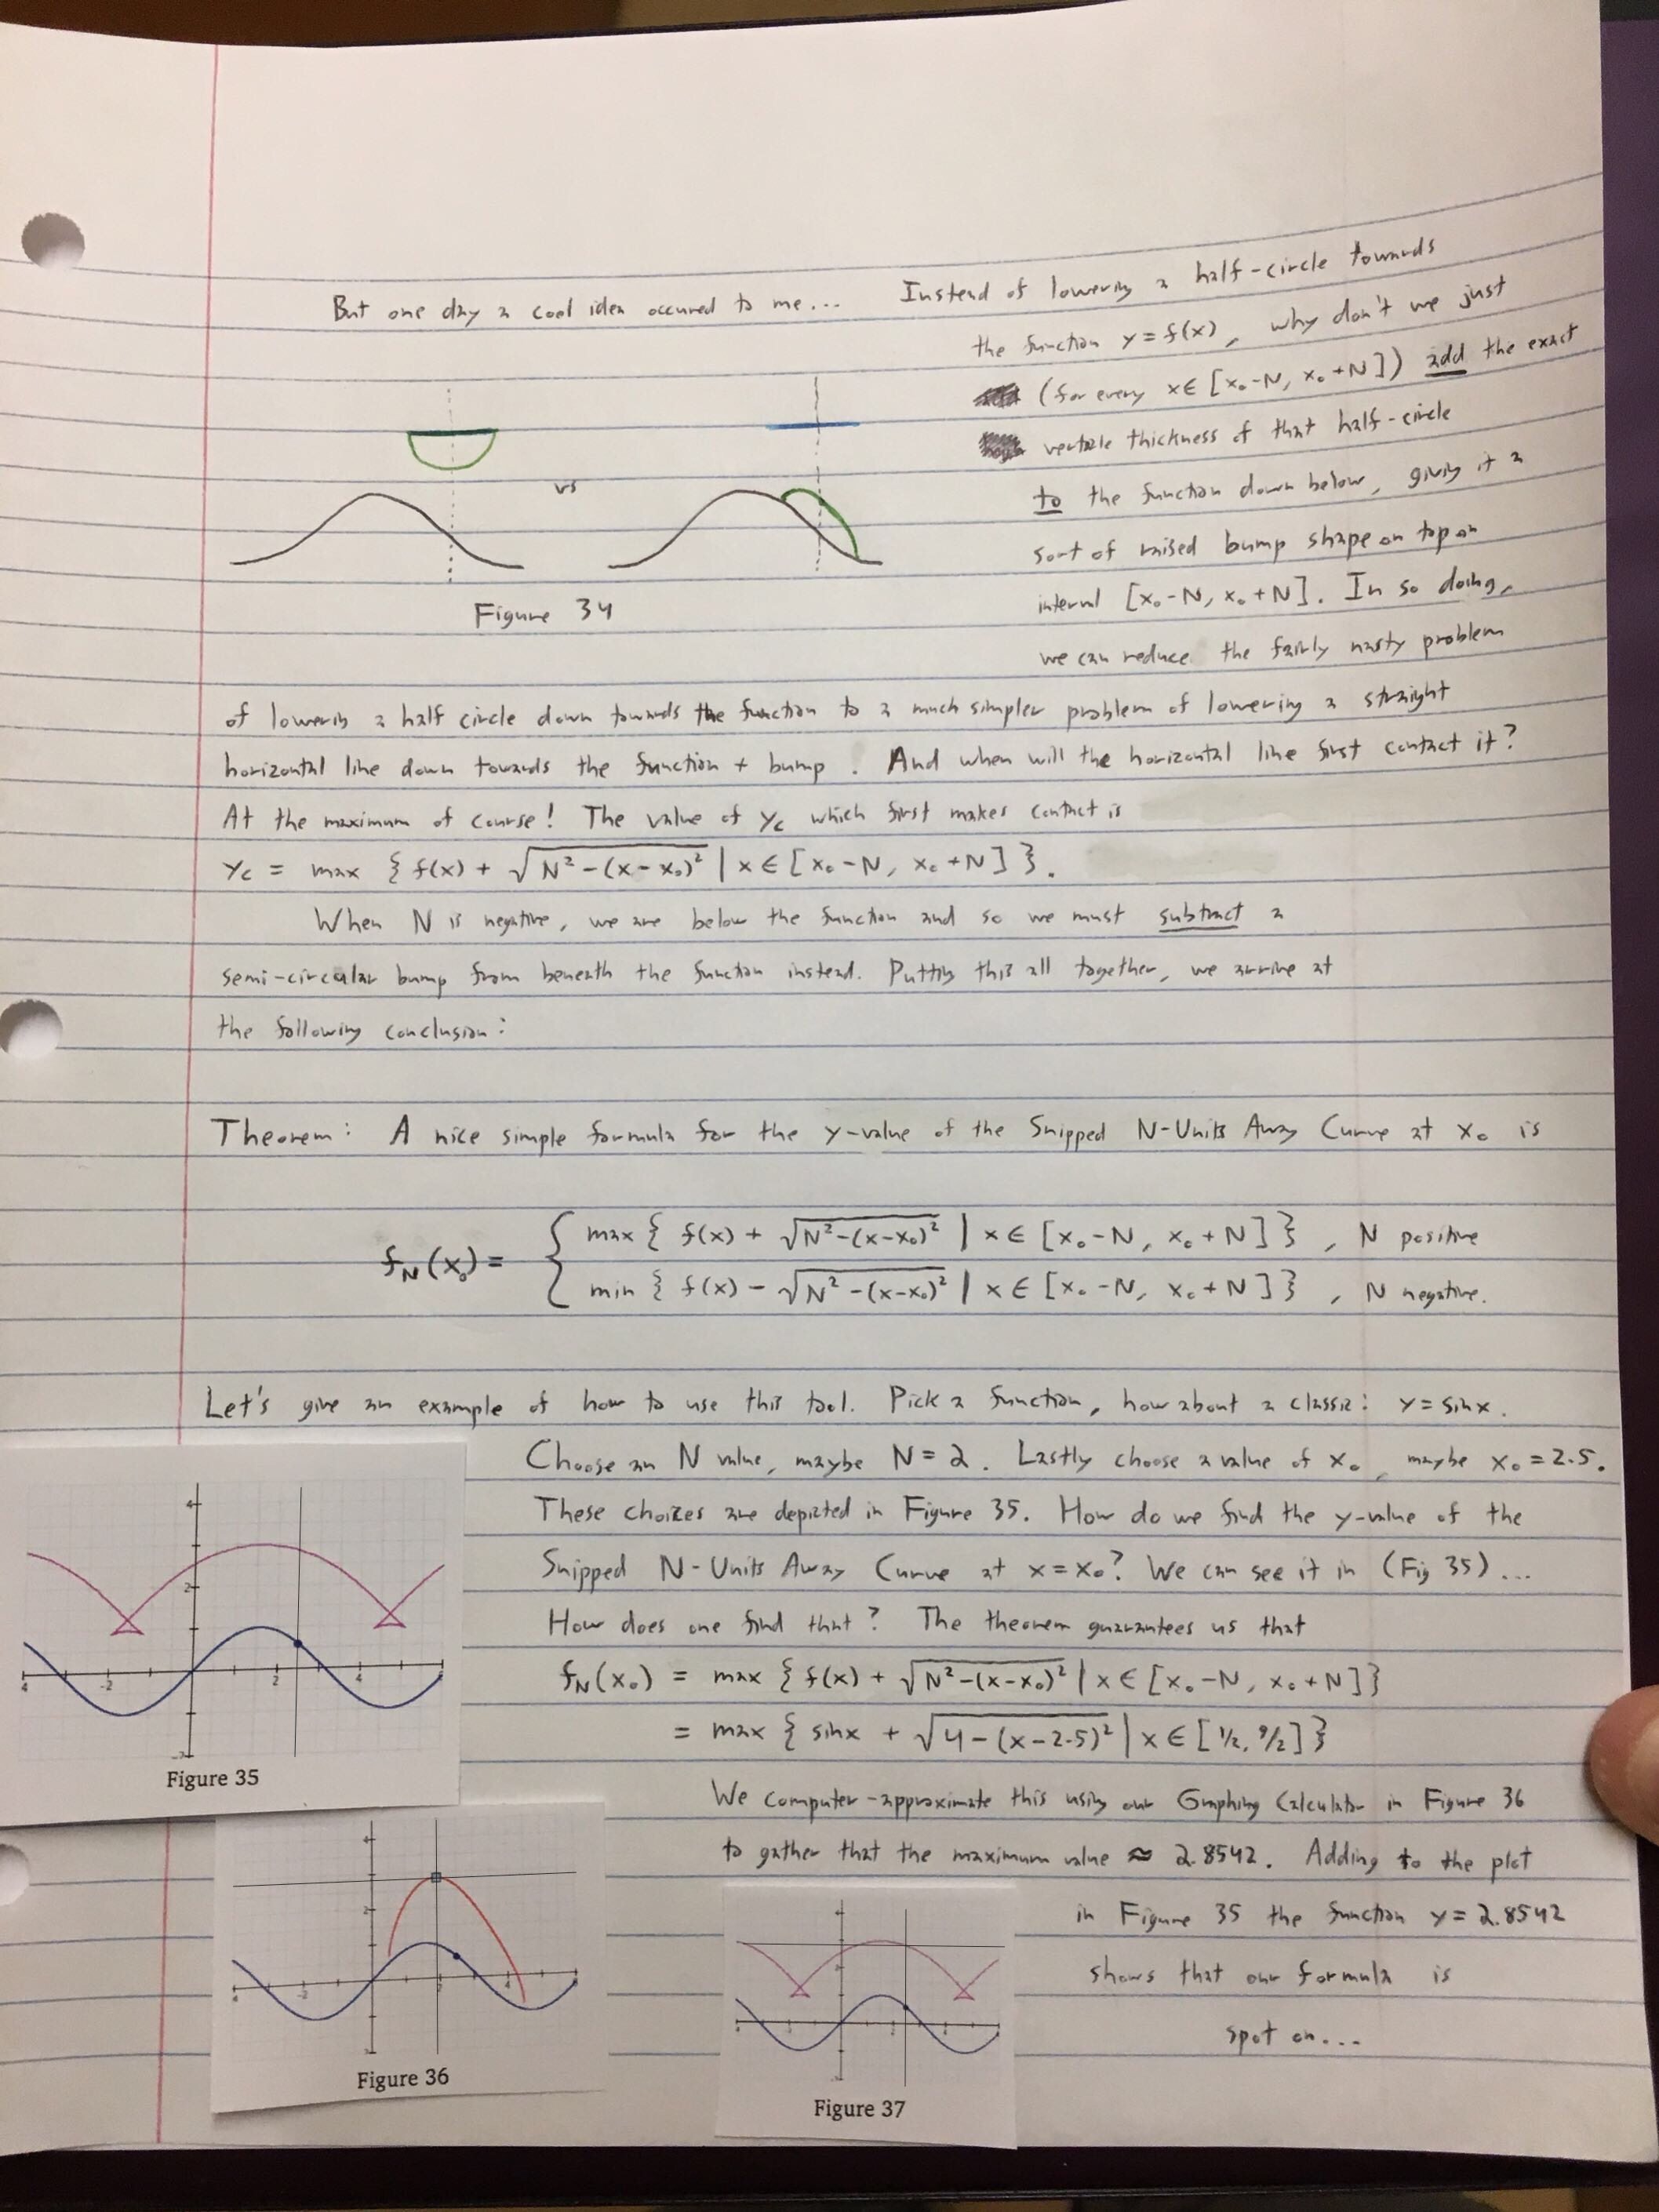
\includegraphics[width=.9\linewidth]{constructed-formula-img/Fig 10-34.png}
  \caption{Caption}
  \label{fig:fig10-34}
\end{wrapfigure}

But one day a cool idea occurred to me. Instead of lowering a half-circle towards the function $y = f(x)$, why don't we just (for every $x \in [x_o - N, x_o + N]$), \textit{add} the exact vertical thickness of that half-circle \textit{to} the function down below, giving it a sort of raised bump shape on top on interval $[x_o - N, x_o + N]$. In so doing, we can reduce the fairly nasty problem of lowering half a circle down towards the function to a much simple problem of lowering a straight horizontal line down towards the function + bump. And when will the horizontal line first contact it?

At the maximum of course! The value of $y_c$ which first makes contact it $y_c = max \{ f(x) + \sqrt{N^2 - (x - x_o)^2} | x \in [ x_o - N, x_o + N] \}$.

When $N$ is negative, we are below the function and so we must \textit{subtract} a semi-circular bump from beneath the function instead. Putting this all together, we arrive at the following conclusion:

\begin{myTrm} A nice simple formula for the $y$-value at the Snipped $N$-Units Away Curve at $x_o$ is

$$
f_N(x_o) = \begin{cases}
 max \{ f(x) + \sqrt{N^2 - (x - x_o)^2} | x \in [ x_o - N, x_o + N] \}, & N > 0 \\
 min \{ f(x) - \sqrt{N^2 - (x - x_o)^2} | x \in [ x_o - N, x_o + N] \}, & N < 0
\end{cases}
$$

\end{myTrm}

Let's give an example of how to use this tool. Pick a function, how about a classical $y = sin x$?. Choose an $N$ value, maybe $N = 2$. Lastly choose a value of $x_o$, maybe $x_o = 2.5$. These choices are depicted in Figure $\ref{fig:fig10-35}$. How do we find the $y$-value of the Snipped $N$-Units Away Curve at $x = x_o$? We can see it in (Fig $\ref{fig:fig10-35}$... 

How does one find that? The theorem guarantees us that $f_N(x_o) = max \{ f(x) + \sqrt{N^2 - (x - x_o)^2} | x \in [ x_o - N, x_o + N] \} = max \{ sin x + \sqrt{4 - (x - 2.5)^2} | x \in [\dfrac{1}{2}, \dfrac{9}{2}]\}$. We computer-approximate this using a Graphic Calculator in Figure $\ref{fig:fig10-36}$ to gather that the maximum value $\approx 2.8542$. Adding to the plot in Figure $\ref{fig:fig10-35}$ the function $y = 2.8542$ shows that our formula is spot on...

\begin{figure}[H]
    \centering
    \begin{minipage}[b]{0.3\linewidth}
        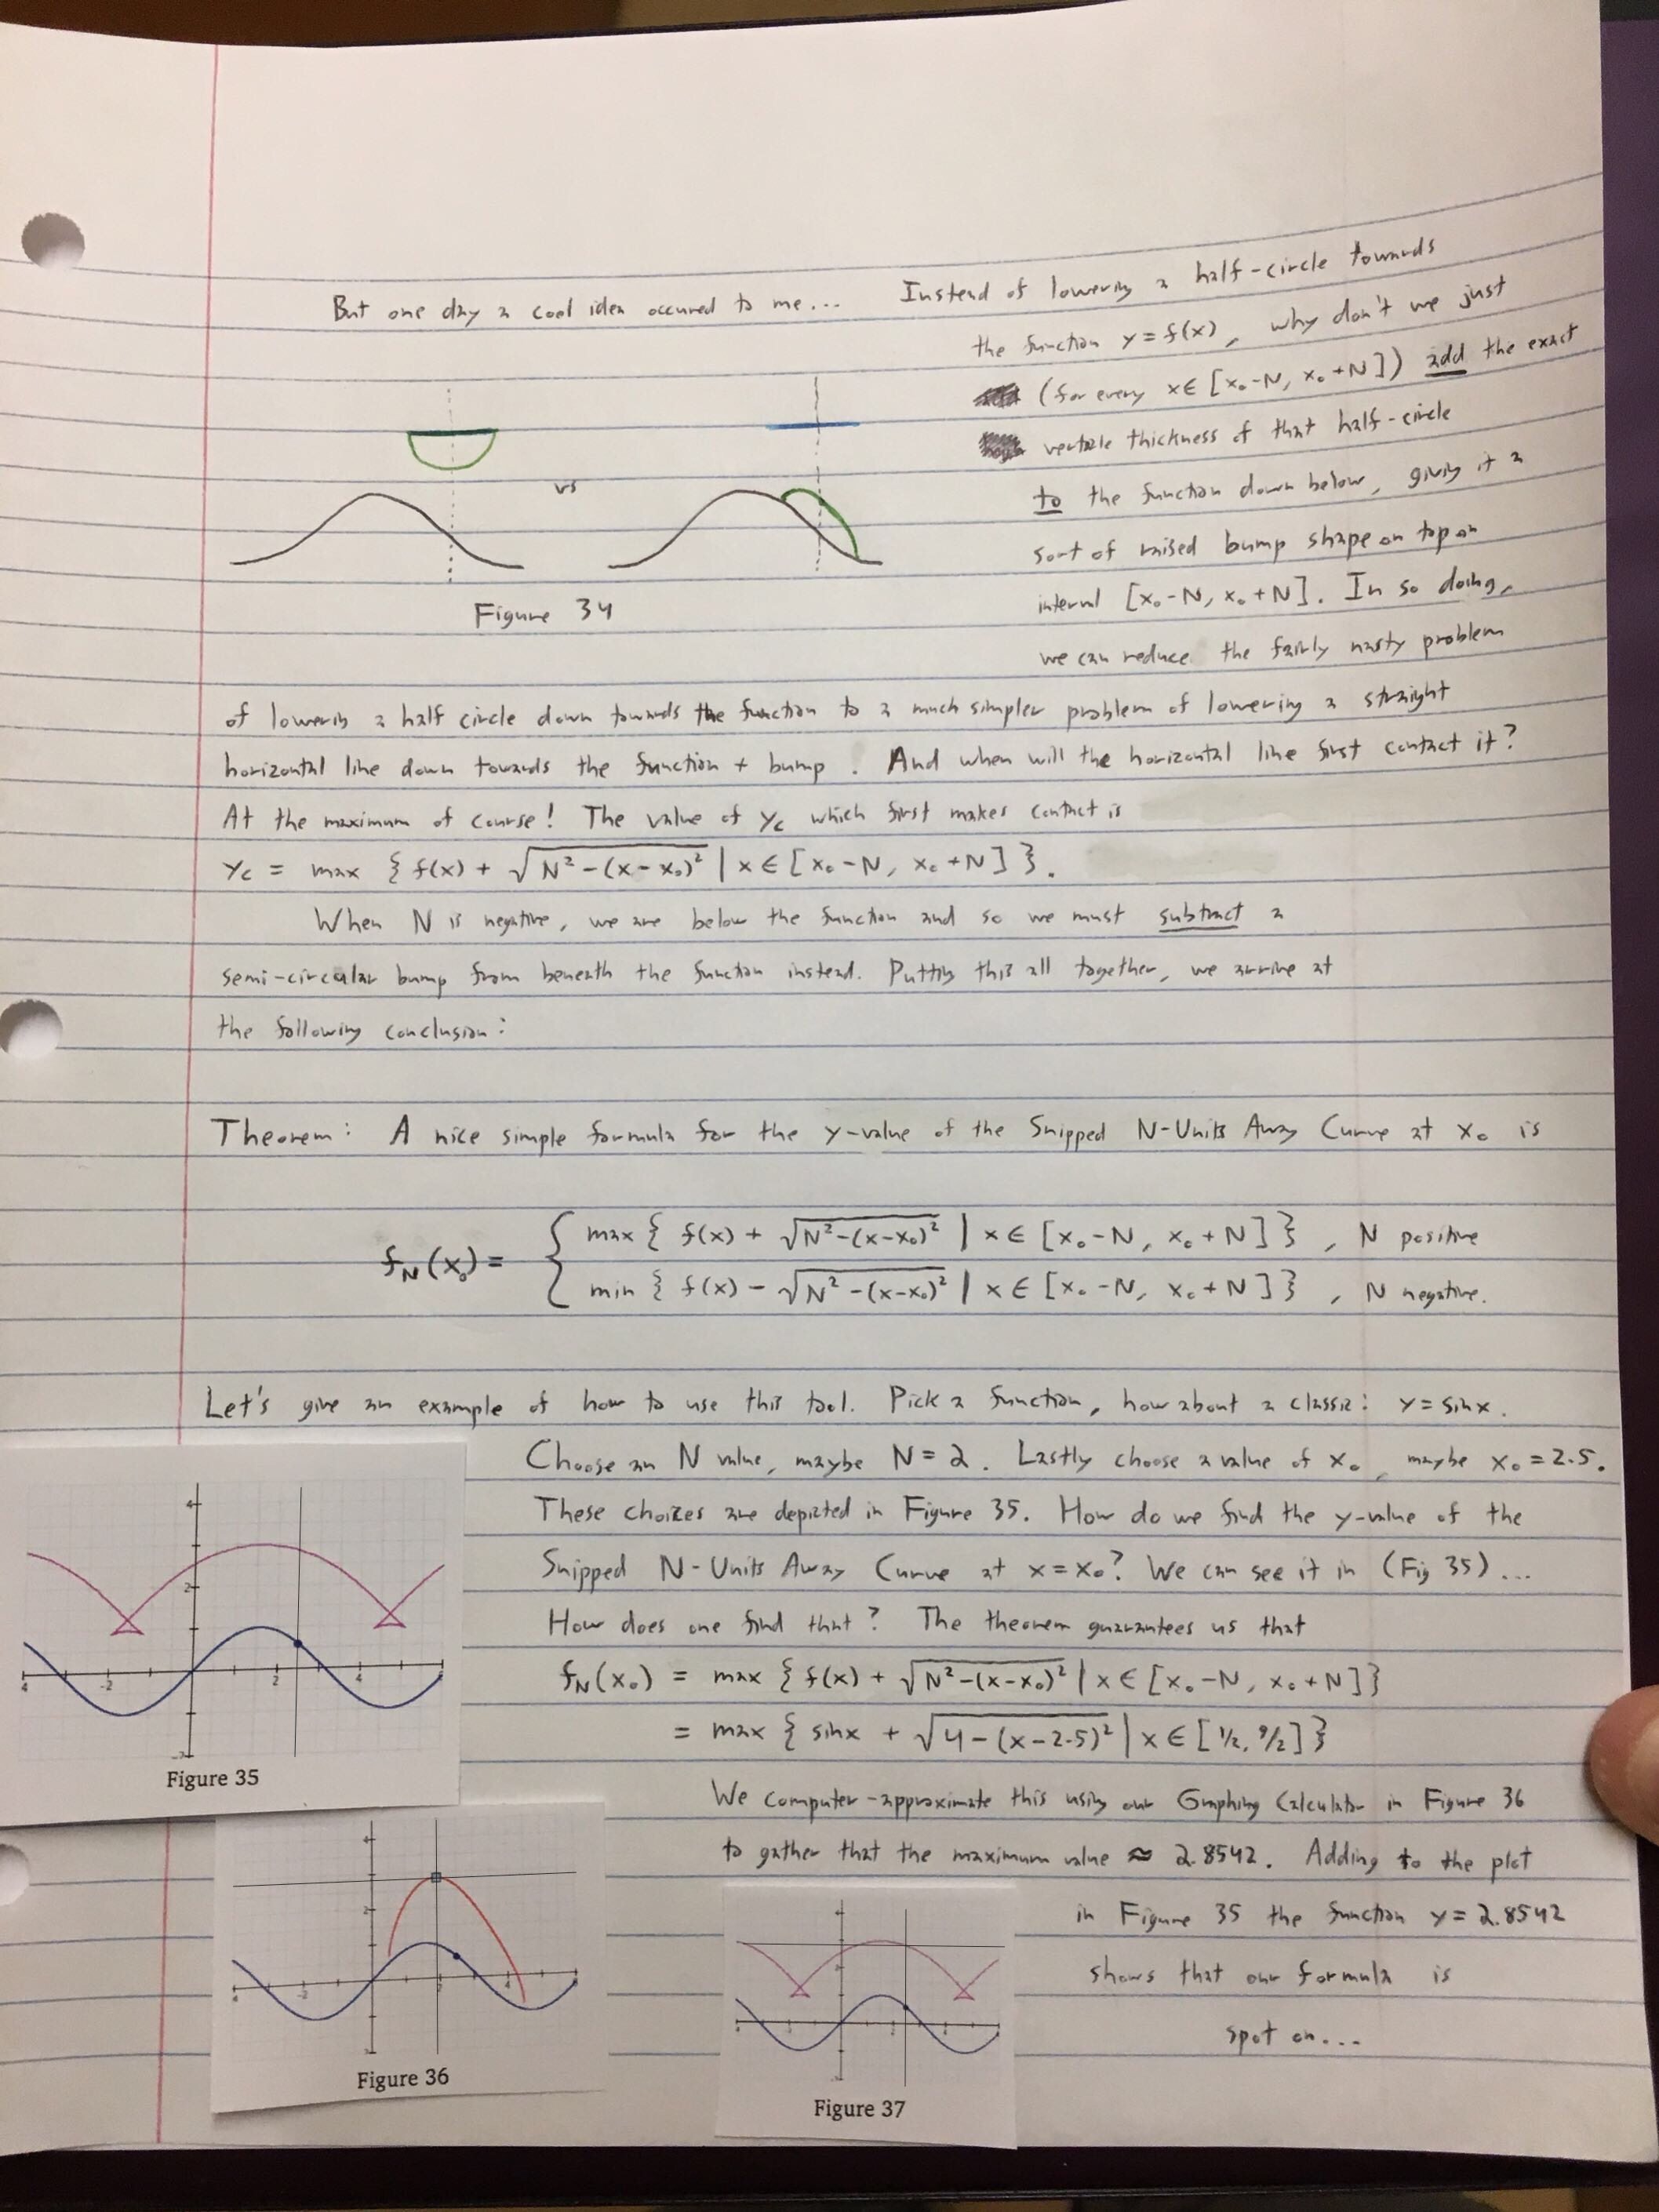
\includegraphics[width = .9\linewidth]{constructed-formula-img/Fig 10-35.png}
        \caption{Caption}
        \label{fig:fig10-35}
    \end{minipage}
    \begin{minipage}[b]{0.3\linewidth}
        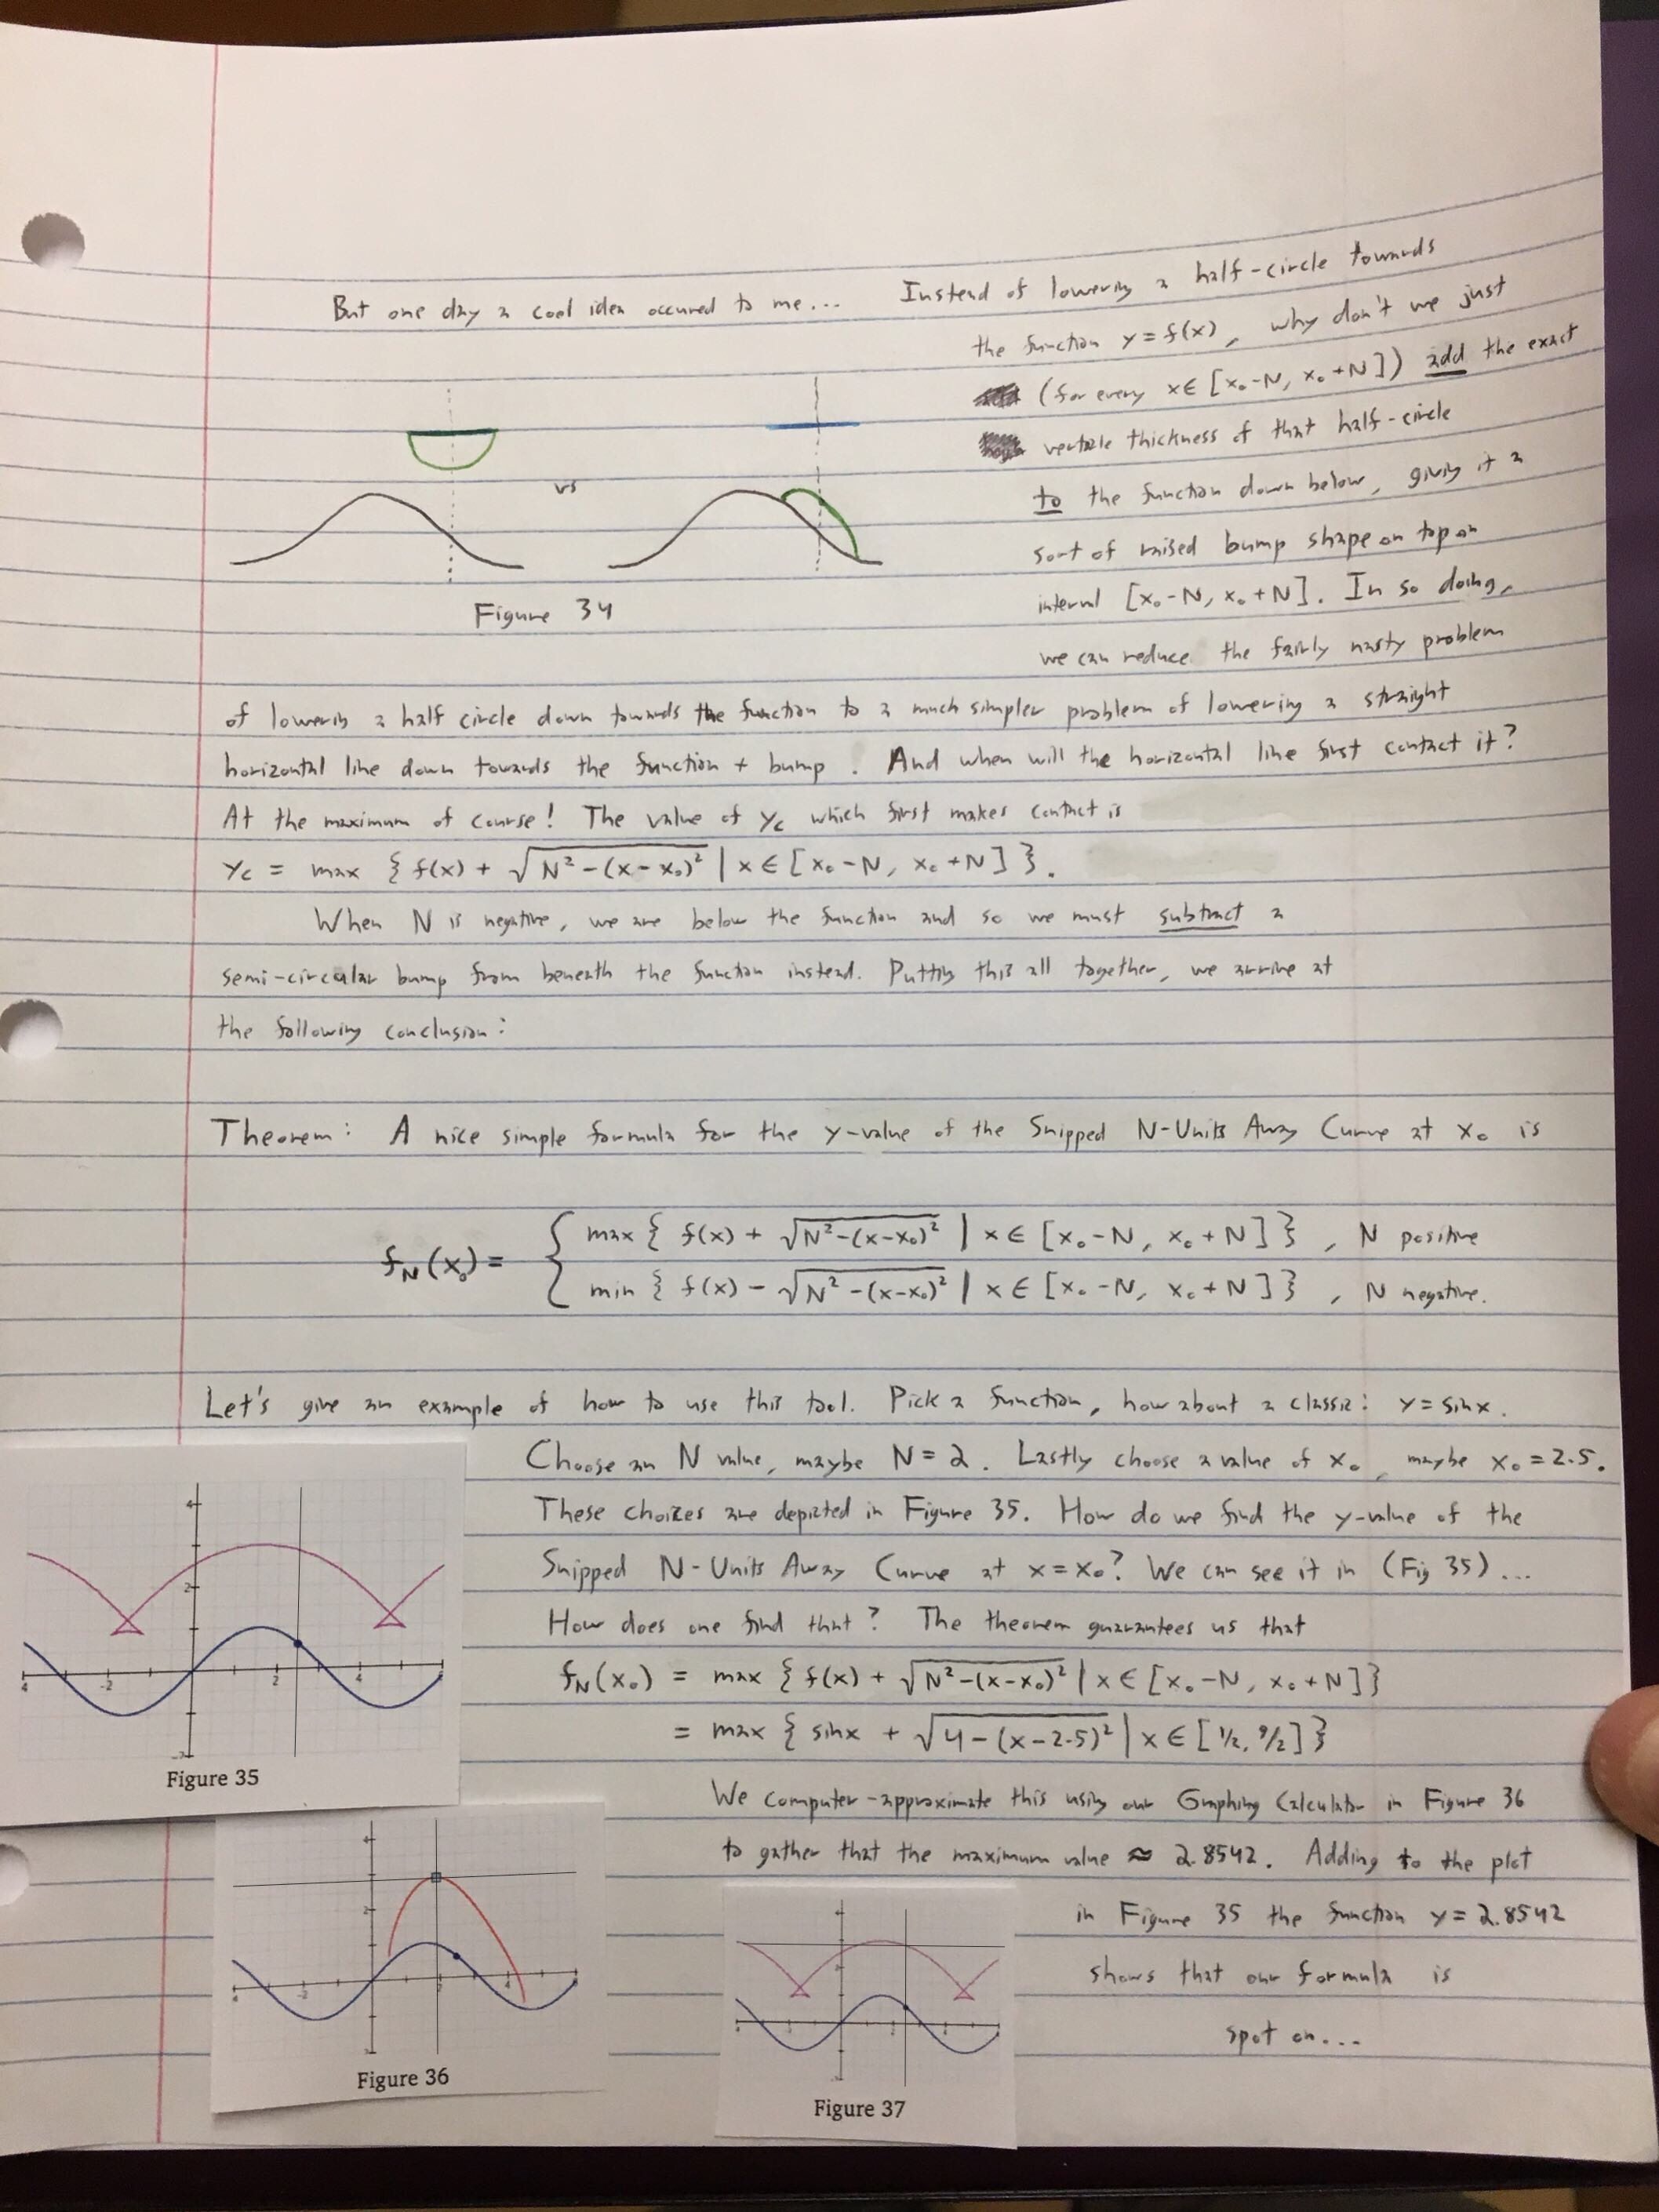
\includegraphics[width = .9\linewidth]{constructed-formula-img/Fig 10-36.png}
        \caption{Caption}
        \label{fig:fig10-36}
    \end{minipage}
    \begin{minipage}[b]{0.3\linewidth}
        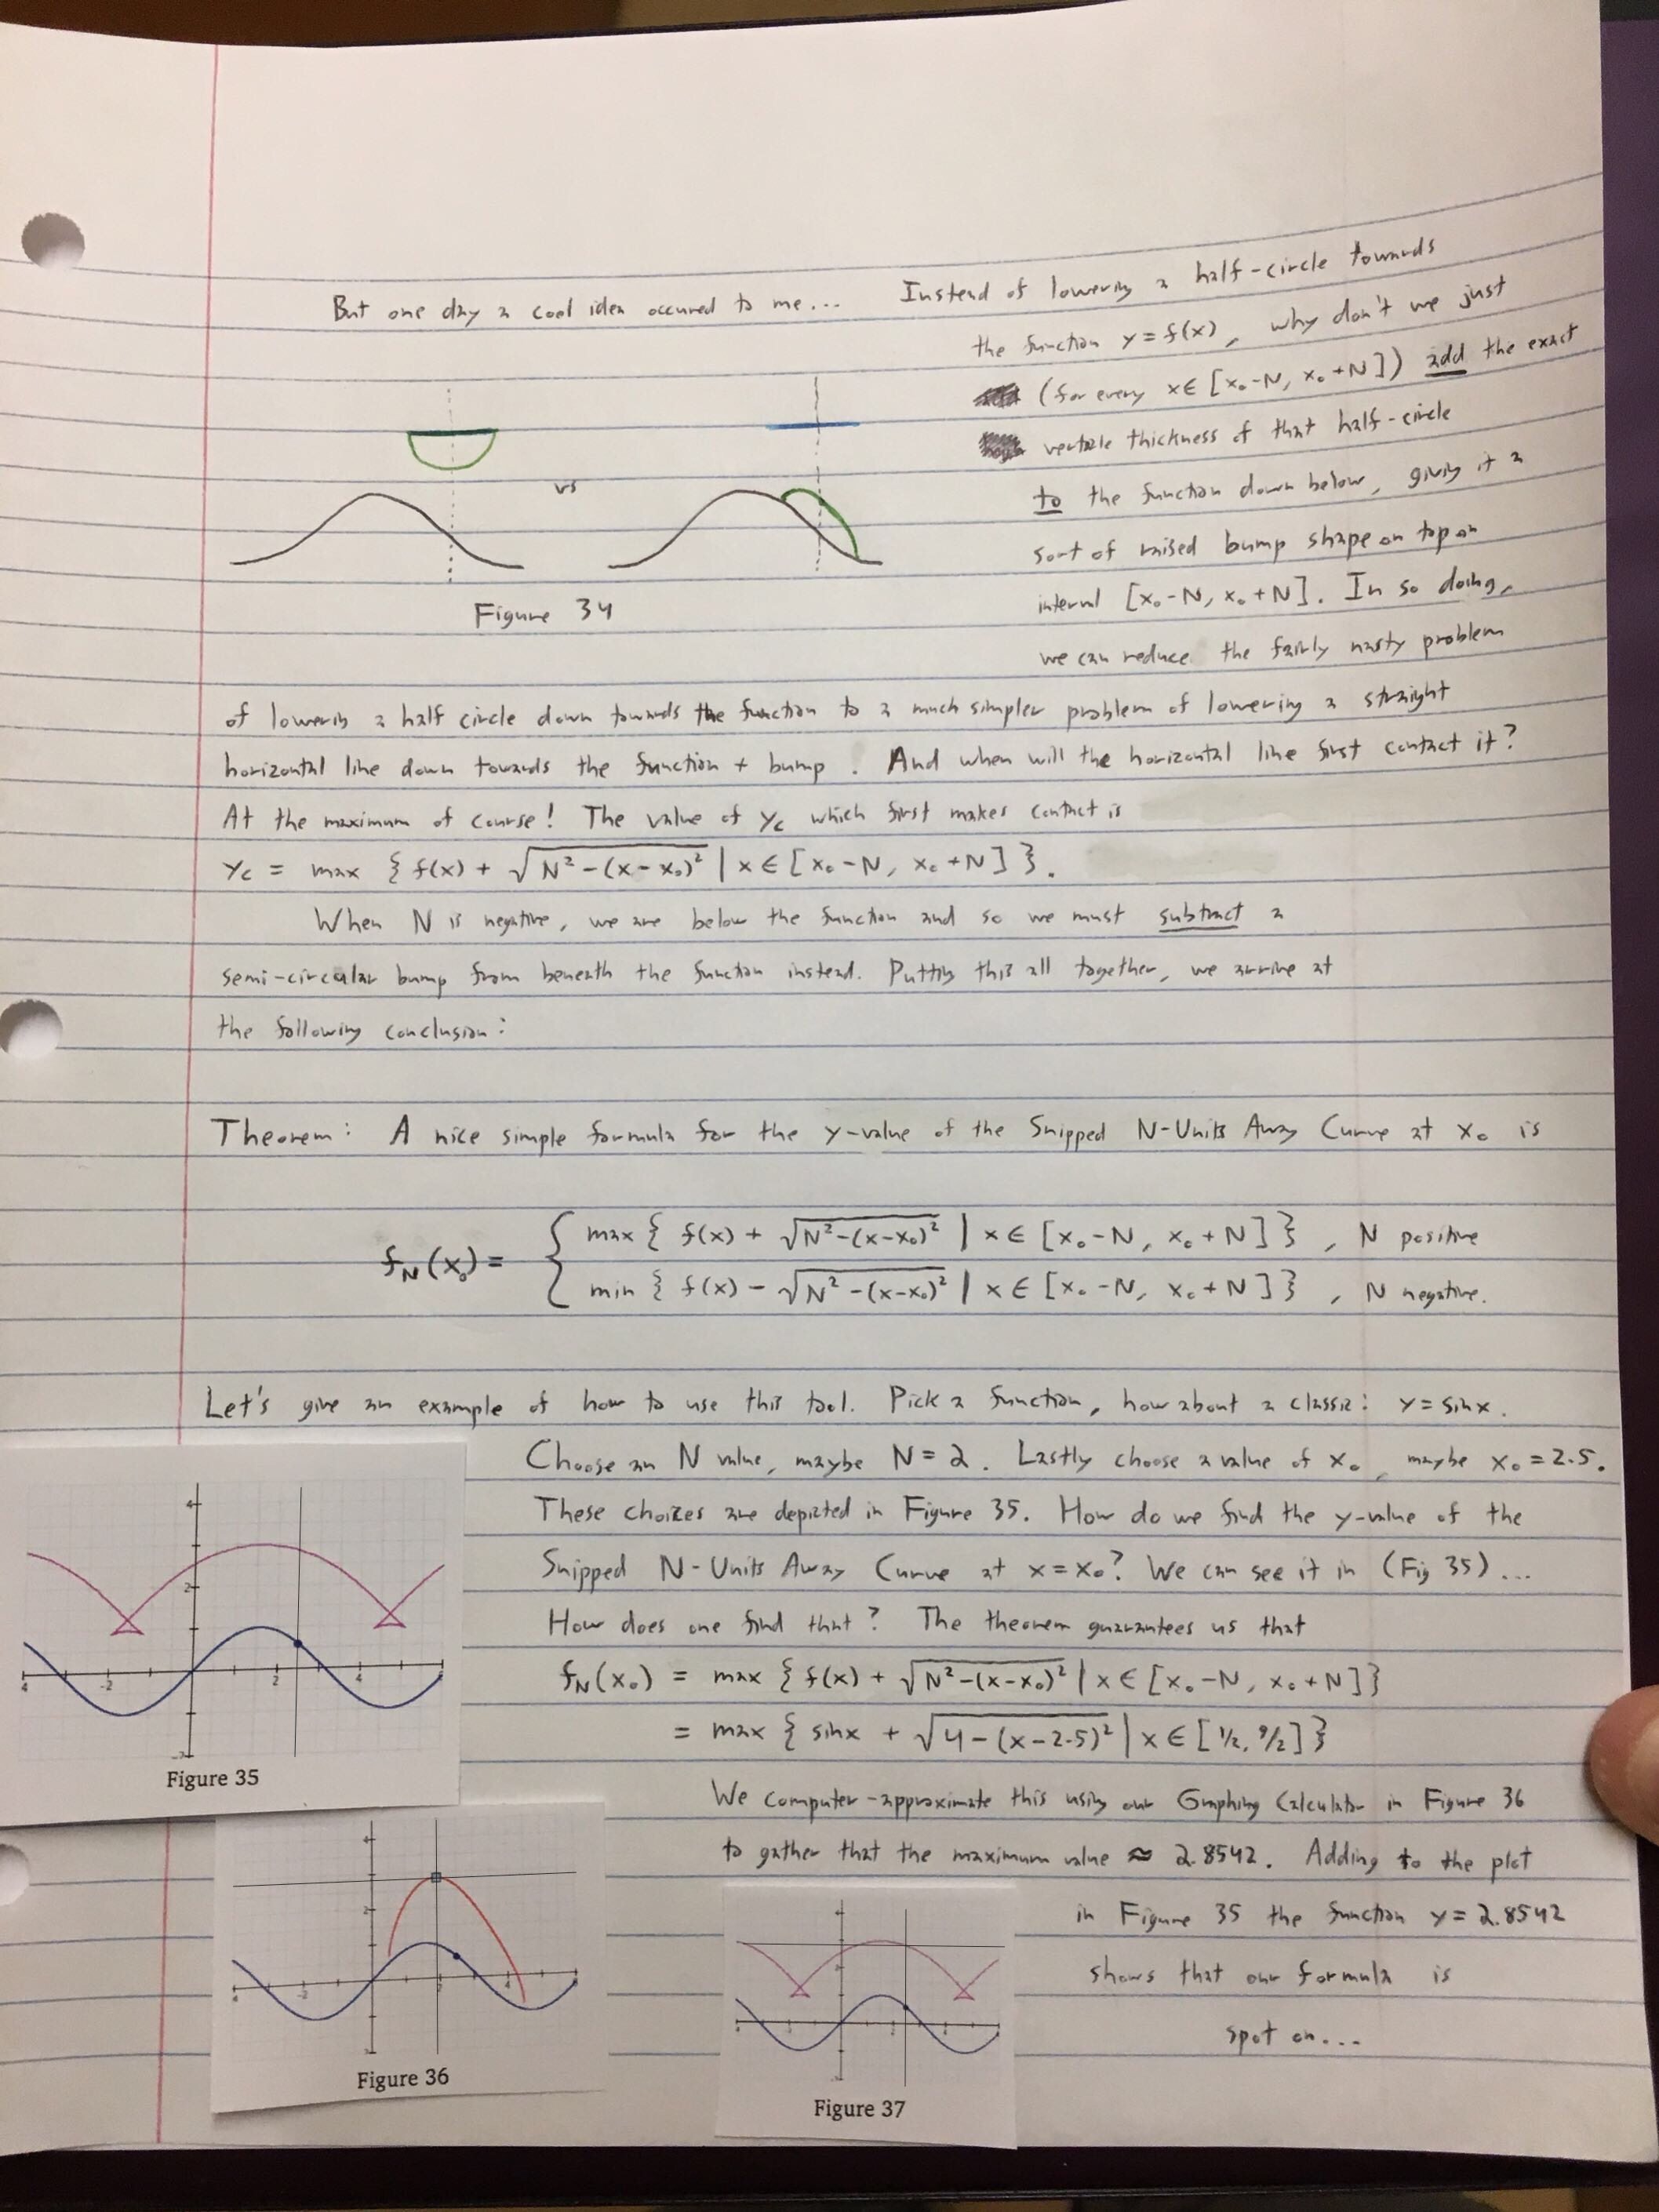
\includegraphics[width = .9\linewidth]{constructed-formula-img/Fig 10-37.png}
        \caption{Caption}
        \label{fig:fig10-37}
    \end{minipage}
\end{figure}